\documentclass[crop,tikz]{standalone}% 'crop' is the default for v1.0, before it was 'preview'
%\usetikzlibrary{...}% tikz package already loaded by 'tikz' option
\usepackage{color}
\usepackage{siunitx}

\begin{document}
\fontfamily{cmss}
{ \begin{tikzpicture}
    \node(a) at (0,0){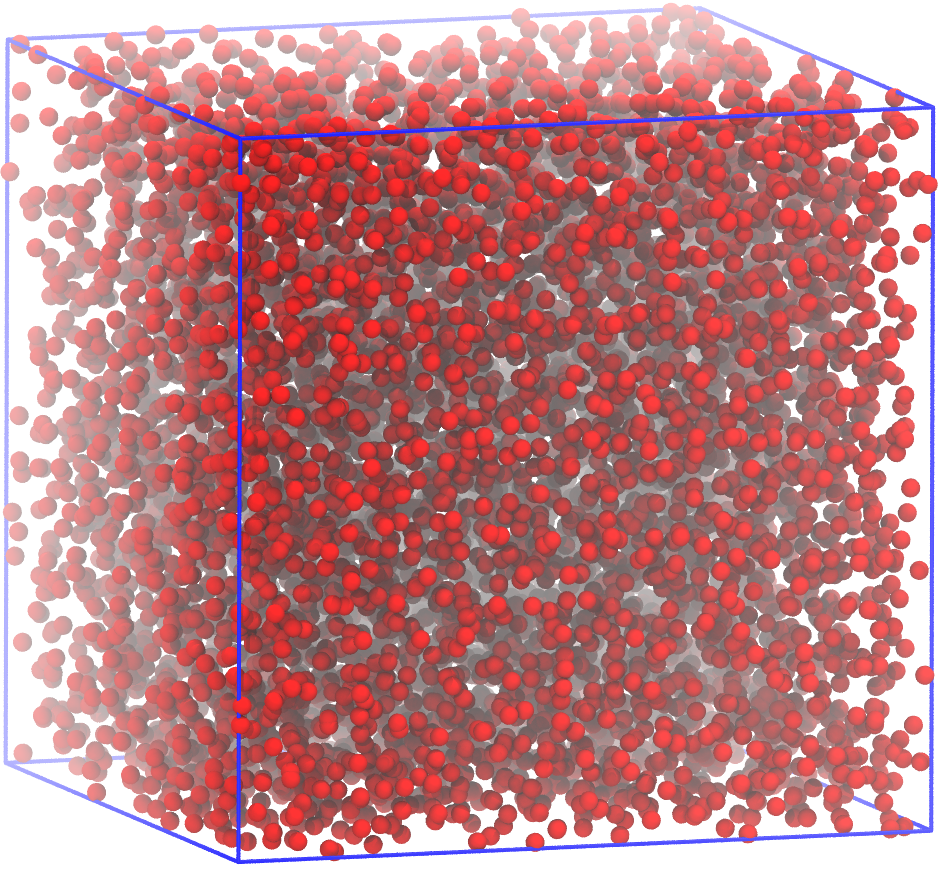
\includegraphics[width=1.2in]{waterbox.png}};    

    
    \node(b) at (4.5,0){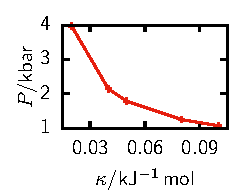
\includegraphics{p_kappa_water.pdf}};    
    \draw[->,thick] (a) -- ([xshift=-2cm]b|-  a)  node[midway,above]{$NVT$} node[midway,below]{$\textcolor{blue}{a}=0$};
       
    
    \node[label={[yshift=-0.4cm,xshift=0.5cm]\textcolor{blue}{$a$} required for \SI{1}{bar}}](c) at (0,-3.75){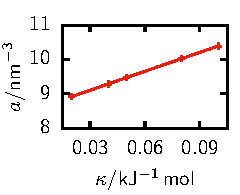
\includegraphics{a_kappa_water.pdf}};

  %   \draw[->,thick] ([xshift=0.5cm,yshift=0.5cm]b.south west) -- ([xshift=-0.4cm,yshift=-0.3cm]c.north east);

     \node[label={[yshift=-0.4cm,xshift=0.5cm] $NPT$ equilibration}](d) at (4.5,-3.75){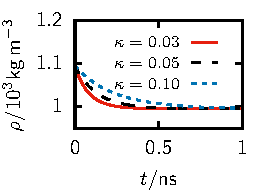
\includegraphics{dens_kappa_water.pdf}};
  %   \draw[->,thick] ([xshift=-3cm]c) -- ([xshift=-3cm]d|-  c)  node[midway,above]{$NPT$};


     \node[anchor=north west,opacity=0.75,text opacity=1,fill=white] (A) at ([yshift=-0.cm,xshift=-0.6cm]a.north west){\Large A};
     \node[anchor=north west,opacity=0.75,text opacity=1,fill=white] (B) at ([yshift=-0.cm,xshift=-0.1cm]b.north west){\Large B};
     \node[anchor=north west,opacity=0.75,text opacity=1,fill=white] (C) at ([yshift=0.2cm,xshift=-0.1cm]c.north west){\Large C};
     \node[anchor=north west,opacity=0.75,text opacity=1,fill=white] (D) at ([yshift=0.2cm,xshift=-0.1cm]d.north west){\Large D};
    %% \node(e) at (0,-6){\(P_{0,\mu}=\frac 1V \int\text d \textbf r~\frac{1}{\rho_0}\frac{1}{2\kappa}\left(\phi(\textbf r)^2-\textcolor{blue}{a}^2\right)\)};
    %% \draw[gray,thick,rounded corners] ([yshift=-0.0cm]e.north west) rectangle ([yshift=-0.cm]e.south east);
  \end{tikzpicture}}
\end{document}
